\documentclass[a4paper,12pt]{article}
\usepackage{fontspec}
\usepackage{xeCJK}
\setCJKmainfont{Noto Serif CJK SC}
\usepackage{geometry,graphicx,fancyhdr,tikz,float,xcolor,amsmath,booktabs,enumitem}
\geometry{left=1in,right=1in,top=1in,bottom=1in}
\usetikzlibrary{positioning,arrows.meta,fit,calc}
\pagestyle{fancy}\fancyhf{}\fancyfoot[C]{\thepage}
\setlength{\parindent}{2em}

\begin{document}

\begin{titlepage}
\centering
\vspace*{2cm}
\Huge{\textbf{深\ 圳\ 大\ 学\ 实\ 验\ 报\ 告}}\\[1.3cm]
{\Large\textbf{课程名称}\quad\underline{\makebox[8cm][c]{Python程序设计}}}\\[0.5cm]
{\Large\textbf{项目名称}\quad\underline{\makebox[8cm][c]{NumPy Image Encoder}}}\\[0.5cm]
{\Large\textbf{学院}\quad\underline{\makebox[8cm][c]{人工智能学院}}}\\[0.5cm]
{\Large\textbf{指导教师}\quad\underline{\makebox[8cm][c]{舒婷}}}\\[0.5cm]
{\Large\textbf{报告人}\quad\underline{\makebox[3cm][c]{金佳圆}}\quad\textbf{学号}\quad\underline{\makebox[3cm][c]{2025221025}}}\\[0.5cm]
{\Large\textbf{实验时间}\quad\underline{\makebox[8cm][c]{2026.11.19}}}\\[0.5cm]
{\Large\textbf{提交时间}\quad\underline{\makebox[8cm][c]{2026.11.22}}}\\[2cm]
\vfill {\Large\textbf{教务处制}}
\end{titlepage}

\section{Objectives}
The objective is to reproduce the forward calculation of the supplied OpenCLIP ViT-B/32 image tower with NumPy. The implementation receives a batch of preprocessed RGB images with shape $[B,3,224,224]$ and returns one normalized 512-dimensional feature vector per image. No learning or parameter update is performed; all model parameters are supplied by the project.

\section{Overview}
The calculation follows the lecture pipeline:
\begin{enumerate}[label=\arabic*.]
\item split each image into 49 ordered $32\times32$ patches and project every patch from 3072 to 768 features;
\item prepend a CLS token, add positional embeddings, and pass the 50-token sequence through 12 Transformer blocks;
\item select the final CLS token, apply post-Norm, project it to 512 dimensions, and normalize it to unit length.
\end{enumerate}

\begin{figure}[H]
\centering
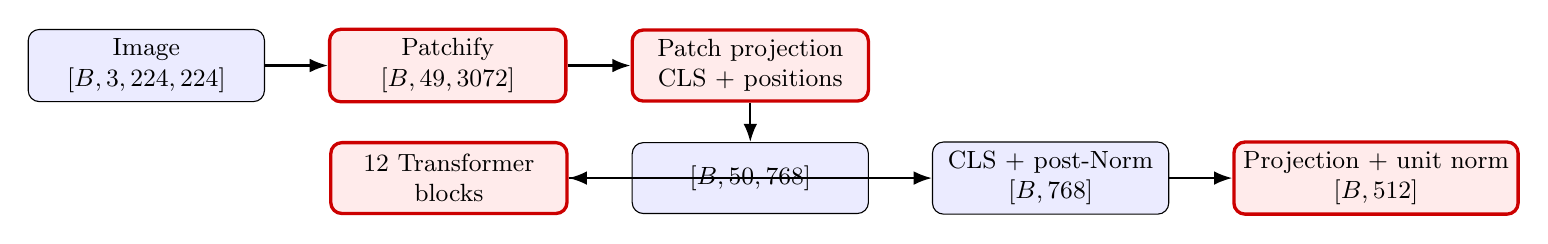
\begin{tikzpicture}[node distance=5mm and 8mm, every node/.style={font=\small,align=center}, box/.style={draw,rounded corners,fill=blue!8,minimum width=30mm,minimum height=9mm}, redbox/.style={box,draw=red!80!black,very thick,fill=red!8}, arrow/.style={-{Latex},thick}]
\node[box] (image) {Image\\$[B,3,224,224]$};
\node[redbox,right=of image] (patch) {Patchify\\$[B,49,3072]$};
\node[redbox,right=of patch] (embed) {Patch projection\\CLS + positions};
\node[box,below=of embed] (tokens) {$[B,50,768]$};
\node[redbox,left=of tokens] (blocks) {12 Transformer\\blocks};
\node[box,right=of tokens] (cls) {CLS + post-Norm\\$[B,768]$};
\node[redbox,right=of cls] (out) {Projection + unit norm\\$[B,512]$};
\draw[arrow] (image)--(patch);\draw[arrow] (patch)--(embed);\draw[arrow] (embed)--(tokens);\draw[arrow] (tokens)--(blocks);\draw[arrow] (blocks)--(cls);\draw[arrow] (cls)--(out);
\end{tikzpicture}
\caption{Implemented NumPy image-encoder pipeline. Red boxes highlight the assessed implementation parts.}
\label{fig:vit}
\end{figure}

\section{Implementations}
The patch operation reshapes $[B,3,224,224]$ into a $7\times7$ patch grid and transposes the axes so that each row is one patch in channel-first order. Multi-head attention reshapes $[B,N,768]$ into $[B,12,N,64]$, computes
\[
S=\frac{QK^T}{\sqrt{64}},\qquad C=\operatorname{softmax}(S),\qquad A=CV,
\]
then merges the heads and applies the output projection. The Transformer block uses the two required residual paths:
\[
r=x+\operatorname{Attention}(\operatorname{Norm}_1(x)),
\qquad y=r+W_2\,\operatorname{GELU}(W_1\operatorname{Norm}_2(r)+b_1)+b_2.
\]
The final projection uses the supplied matrix with layout $[768,512]$; it is therefore multiplied directly without transposition.

\section{Results}
The staged checker was run with `python check.py --stage all`. All stages passed.
\begin{table}[H]
\centering
\begin{tabular}{lccc}
\toprule
Stage & Shape & Maximum absolute error & Mean absolute error\\
\midrule
Preprocess & $(10,3,224,224)$ & $0$ & $0$\\
Patches & $(2,49,3072)$ & $0$ & $0$\\
Input tokens & $(2,50,768)$ & $4.387\times10^{-5}$ & $1.335\times10^{-6}$\\
Block 0 & $(2,50,768)$ & $7.147\times10^{-6}$ & $3.348\times10^{-7}$\\
Last tokens & $(2,50,768)$ & $4.196\times10^{-5}$ & $2.633\times10^{-6}$\\
Output & $(10,512)$ & $5.662\times10^{-7}$ & $8.688\times10^{-8}$\\
Batch & $(3,512)$ & $4.061\times10^{-7}$ & $7.848\times10^{-8}$\\
\bottomrule
\end{tabular}
\caption{Independent FP32 numerical checks.}
\end{table}

\section{Discussion}
The main implementation risk was confusing the stored linear-weight layouts. Attention and MLP weights are stored as $[\text{out},\text{in}]$ and therefore use `.T`, while `visual.proj` is already $[\text{in},\text{out}]$ and must not be transposed. A second issue was preserving `float32`: dividing the attention scores by a default `float64` square root promoted the complete Transformer calculation, so the scale was explicitly converted to `np.float32`. After this fix, all shape, finite-value, tolerance, and unit-length checks passed. The code can be reproduced with the commands in `README_submission.md`.

\section*{Repository}
The completed source code and report template are available at:\\
\texttt{https://github.com/Auga0123/project1-numpy-image-encoder}

\section*{Contribution and assistance}
I implemented the six NumPy TODO groups, ran the supplied staged numerical checks, and prepared the report and reproduction instructions. Assistance was used for understanding the provided project structure, array shapes, and debugging the numerical dtype issue.

\end{document}
